% Tipe dokumen adalah report dengan satu kolom kertas A4 satu sisi.
% Ukuran font 12pt
\documentclass[12pt, a4paper, onecolumn, oneside, final]{report}

% Load konfigurasi LaTeX untuk tipe laporan thesis
\usepackage{ta}

% Load konfigurasi khusus untuk laporan yang sedang dibuat
%-----------------------------------------------------------------------------%
% Informasi Mengenai Dokumen
%-----------------------------------------------------------------------------%
% 
% Judul laporan. 
\var{\judul}{\textit{Template} \latex~untuk Tugas Akhir Universitas Telkom --- versi 1.1}
% 
% Tulis kembali judul laporan, kali ini akan diubah menjadi huruf kapital
\Var{\Judul}{\textit{Template} \latex~untuk Tugas Akhir Universitas Telkom --- versi 1.1}
% 
% Tulis kembali judul laporan namun dengan bahasa Inggris
\var{\judulInggris}{\latex~Template for Universitas Telkom Undergraduate Thesis --- version 1.1}

\Var{\JudulInggris}{\latex~Template for Universitas Telkom Undergraduate Thesis --- version 1.1}

% 
% Tipe laporan, dapat berisi Skripsi, Tugas Akhir, Thesis, atau Disertasi
\var{\type}{Tugas Akhir}
% 
% Tulis kembali tipe laporan, kali ini akan diubah menjadi huruf kapital
\Var{\Type}{Tugas Akhir}
% 
% Tulis nama penulis 
\var{\penulis}{Gopher Golang's Fan}
\var{\alamat}{Jl. xxx i no. j kkkkkkkk}
\var{\tlp}{08xx662xxxxx}
\var{\email}{aaa@bbb.ccc}
% 
% Tulis kembali nama penulis, kali ini akan diubah menjadi huruf kapital
\Var{\Penulis}{Gopher Golang's Fan}
% 
% Tulis NPM penulis
\var{\nim}{110111xxxx}
% 
% Tuliskan Fakultas dimana penulis berada
\Var{\Fakultas}{Fakultas Teknik Elektro}
\var{\fakultas}{Fakultas Teknik Elektro}
% 
% Tuliskan Program Studi yang diambil penulis
\Var{\Program}{Teknik Telekomunikasi}
\var{\program}{Teknik Telekomunikasi}
% 
% Tuliskan tahun publikasi laporan
\Var{\Tahun}{2015}
% 
% Tuliskan gelar yang akan diperoleh dengan menyerahkan laporan ini
\var{\gelar}{Sarjana Teknik}
% 
% Tuliskan tanggal pengesahan laporan, waktu dimana laporan diserahkan ke 
% penguji/sekretariat
\var{\tanggalPengesahan}{26 Juli 2015} 
% 
% Tuliskan tanggal keputusan sidang dikeluarkan dan penulis dinyatakan 
% lulus/tidak lulus
%\var{\tanggalLulus}{25 April 2015}
% 
% Tuliskan pembimbing 
\var{\pembimbingSatu}{Dr. Awal Tengah Akhir}
\var{\nikSatu}{99xxxxxx-1}
\var{\pembimbingDua}{Dr. Awal Tengah Akhir}
\var{\nikDua}{99xxxxxx-2}
% 
% Alias untuk memudahkan alur penulisan paa saat menulis laporan
\var{\saya}{Penulis}

%-----------------------------------------------------------------------------%
% Judul Setiap Bab
%-----------------------------------------------------------------------------%
% 
% Berikut ada judul-judul setiap bab. 
% Silahkan diubah sesuai dengan kebutuhan. 
% 
\Var{\kataPengantar}{Kata Pengantar}
\Var{\babSatu}{Pendahuluan}
\Var{\babDua}{Tinjauan Pustaka}
\Var{\babTiga}{Menggunakan \latex}
\Var{\babEmpat}{Template \latex~ untuk Tugas Akhir S1 Teknik Telekomunikasi}
\Var{\babLima}{Kesimpulan dan Saran}


% Awal bagian penulisan laporan
\begin{document}

% Sampul Laporan

\begin{titlepage}
    \begin{center}      
        % judul thesis harus dalam 14pt Times New Roman
        \bo{\Judul} \\[0.75cm]
        
        \textit{\bo{\JudulInggris}} \\[1.0cm]

        \vspace*{1 cm}    
        % harus dalam 14pt Times New Roman
        %\bo{\Type}
        \textbf{TUGAS AKHIR}
        
        \vspace*{1 cm}
        
		Disusun dalam rangka memenuhi salah satu persyaratan untuk menyelesaikan\\
		Program Studi Strata 1 \program

        \vspace*{1 cm}       
        % penulis dan npm
        Disusun oleh:\\
        \bo{\Penulis} \\
        \bo{\nim} \\

        \vspace*{1.0cm}
        
        \begin{figure}
            \begin{center}
                
\includegraphics[scale=1]{pics/Untel.jpg}
            \end{center}
        \end{figure}
        \vspace*{1.0cm}
        % informasi mengenai fakultas dan program studi
        \bo{
        	\Fakultas\\
        	UNIVERSITAS TELKOM\\
        	BANDUNG \\
        	\Tahun
        }
    \end{center}
\end{titlepage}


\pagenumbering{gobble}
% Halaman pengesahan
\addChapter{LEMBAR PENGESAHAN}
\chapter*{}

\AddToShipoutPicture*{%
\gradientbox{white}{white}{%

\begin{minipage}[ct][0.98\paperheight][t]{\paperwidth}%
        \begin{figure}
        		\hspace{1 cm}
%        		\vspace{10 cm}
%            \begin{center}
                
\includegraphics[scale=0.4]{pics/pengesahan_header.png}
%            \end{center}
        \end{figure}
\end{minipage}}}

    \begin{center}
    \textbf{LEMBAR PENGESAHAN}\\
    \textbf{TUGAS AKHIR}\\

	\vspace*{1 cm}

    \textbf{\Judul}\\
    \textit{\textbf{\JudulInggris}}\\
    
	\vspace*{1 cm}
    
    \bo{
    Telah disetujui dan disahkan sebagai Tugas Akhir II\\
    		Program S1 \program\\
        	\fakultas\\
        	Universitas Telkom\\
        	Bandung \\
    }
    
	\vspace*{1.0cm}    
    
    Disusun oleh:\\
    	\vspace*{0.5 cm} 
    \bo{\penulis} \\
    \bo{\nim} \\

    \vspace*{1.0cm}
    \textbf{Bandung, \tanggalPengesahan\\
    Menyetujui,}
    \end{center}
    
    \begin{tabular}{>{\centering\arraybackslash} p{0.3\paperwidth} >{\centering\arraybackslash} p{0.3\paperwidth}}\\
    Pembimbing I & Pembimbing II \\ [2 cm]
    \uline{\pembimbingSatu} & \uline{\pembimbingDua} \\
    \nikSatu & \nikDua
    \end{tabular}
 
    

% Halaman pernyataan orisinalitas
\addChapter{LEMBAR PERNYATAAN ORISINALITAS}
\chapter*{}

\AddToShipoutPicture*{%
\gradientbox{white}{white}{%

\begin{minipage}[ct][0.98\paperheight][t]{\paperwidth}%
        \begin{figure}
        		\hspace{1 cm}
%        		\vspace{10 cm}
%            \begin{center}
                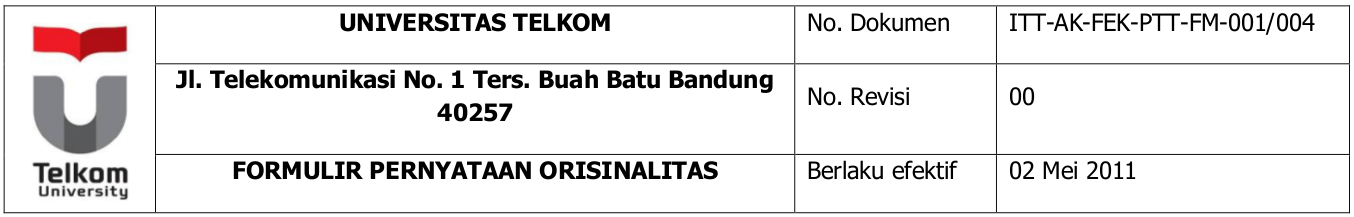
\includegraphics[scale=0.4]{pics/orisinalitas_header.png}
%            \end{center}
        \end{figure}
\end{minipage}}}

    \begin{center}
    \textbf{LEMBAR PERNYATAAN ORISINALITAS}\\
    \end{center}
    
    \begin{tabular}{ll}
    Nama & :\hspace*{0.2 cm}\penulis \\
    NIM & :\hspace*{0.2 cm}\nim \\
    Alamat & :\hspace*{0.2 cm}\alamat \\
    No. Telepon & :\hspace*{0.2 cm}\tlp \\
    Email & :\hspace*{0.2 cm}\email \\
    \end{tabular}
    
    \vspace*{1 cm}
    Menyatakan bahwa Tugas Akhir II ini merupakan karya orisinal saya sendiri, dengan judul :
    
    \begin{center}
    \textbf{\Judul}\\
    \textit{\textbf{\JudulInggris}}\\
    \end{center}
    
    Atas pernyataan ini, saya siap menanggung resiko\slash sanksi yang dijatuhkan kepada saya apabila kemudian ditemukan adanya pelanggaran terhadap kejujuran akademik atau etika keilmuan dalam karya ini, atau ditemukan bukti yang menunjukkan ketidakaslian karya ini.
    
    \vspace*{1 cm}
    
    \begin{tabular}{cl}
    \multirow{6}{*}{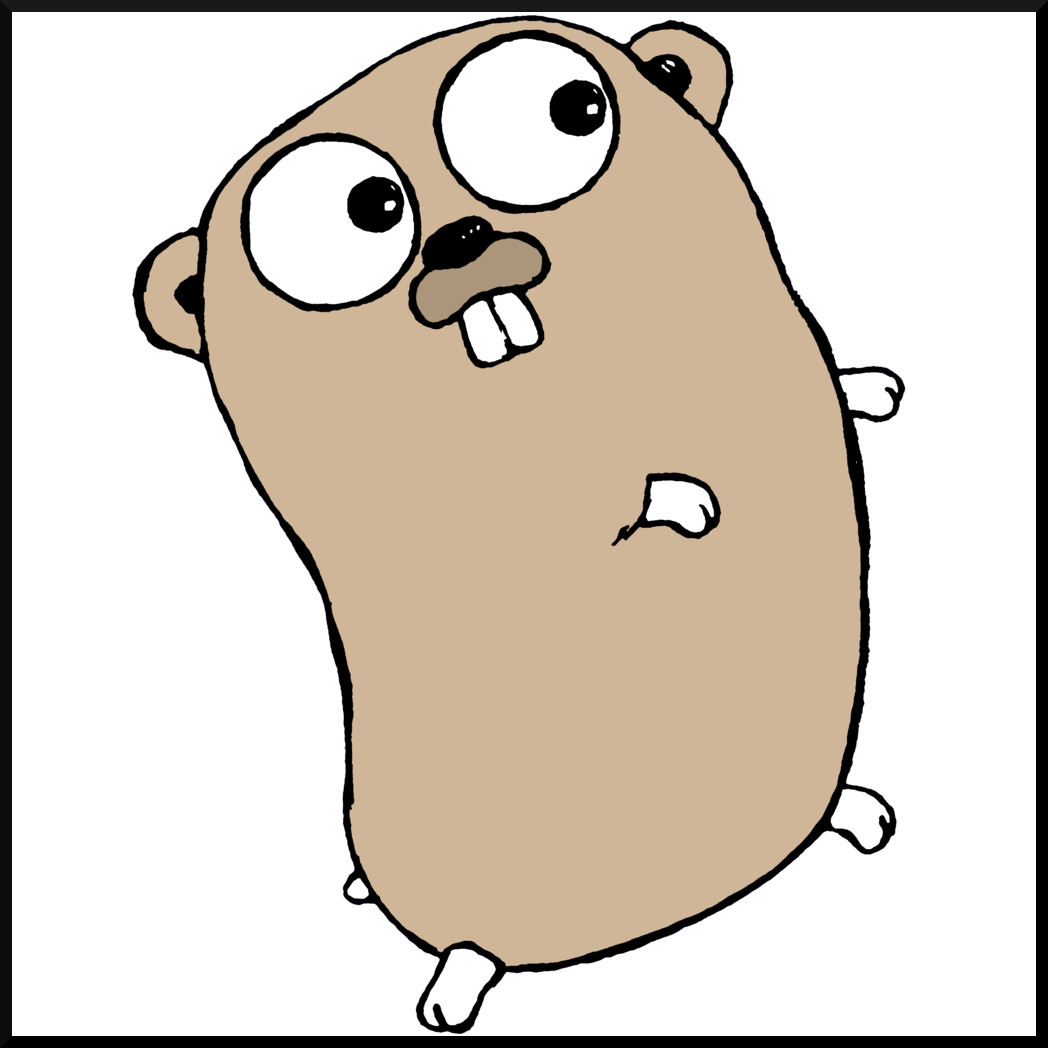
\includegraphics[scale=0.6]{pics/foto.jpg}\hspace{4 cm}}
    & Bandung, \tanggalPengesahan \\
    & \\
    & \\
    & \penulis \\
    \cline{2-2}
    &  \nim\\
    \end{tabular}

% Gunakan penomoran halaman romawi
\pagenumbering{roman}

% setelah bagian ini, halaman dihitung sebagai halaman ke 2
\setcounter{page}{4}

% Abstrak Bahasa Indonesia dan Bahasa Iggris
\addChapter{ABSTRAK}

\chapter*{Abstrak}
\vspace*{0.7cm}

\noindent Abstrak ini\\

\todo{tulis abstrak di sini}

\vspace*{0.2cm}

\noindent Kata Kunci: \textit{kata kunci 1}, \textit{kata kunci 2}, \textit{kata kunci 3}, \textit{kata kunci 4}, \textit{kata kunci 5}\\ 

\newpage

\chapter*{ABSTRACT}
\vspace*{0.7cm}

\noindent This is abstract\\

\todo{write your abstract here}
\vspace*{0.2cm}

\noindent Keywords: keyword 1, keyword 2, keyword 3, keyword 4, keyword 5\\ 

\newpage

% Kata Pengantar
\addChapter{\kataPengantar}
%-----------------------------------------------------------------------------%
\chapter*{\kataPengantar}
%-----------------------------------------------------------------------------%
Kata Pengantar

\todo{tulis kata pengantarmu di sini}
 
\vspace*{0.1cm}
\begin{flushright}
Bandung, \tanggalPengesahan\\[0.1cm]
\vspace*{1cm}
\penulis

\end{flushright}

%\addChapter{UCAPAN TERIMA KASIH}
%%-----------------------------------------------------------------------------%
\chapter*{Ucapan Terima Kasih}
%-----------------------------------------------------------------------------%
\todo{lalalal} 

\vspace*{0.1cm}
\begin{flushright}
Bandung, 1 April 2015\\[0.1cm]
\vspace*{1cm}
\penulis

\end{flushright}

% Daftar isi, gambar, dan tabel
\tableofcontents
\clearpage
\listoffigures
\clearpage
\listoftables
\clearpage
% Daftar Lampiran
\addChapter{DAFTAR LAMPIRAN}
%-----------------------------------------------------------------------------%
\chapter*{Daftar Lampiran}
%-----------------------------------------------------------------------------%
\noindent
Lampiran A: Data Hasil Pengukuran\\
Lampiran B: Kode Program

% Gunakan penomeran Arab (1, 2, 3, ...) setelah bagian ini.
\pagenumbering{arabic}

% Bab 1 : Pendahuluan
%-----------------------------------------------------------------------------%
\chapter{\babSatu}
%-----------------------------------------------------------------------------%
%-----------------------------------------------------------------------------%
\section{Latar Belakang}
%-----------------------------------------------------------------------------%
\todo{Ceritakan latar belakang penelitian ini.}


%-----------------------------------------------------------------------------%
\section{Permasalahan}
%-----------------------------------------------------------------------------%
\todo{Jabarkan rumusan masalah yang dibahas di penelitian ini.}

Berdasarkan latar belakang tersebut, maka rumusan masalah dari tugas akhir ini adalah sebagai berikut:
\begin{enumerate}
\item Bagaimana cara kerja sistem untuk xxx yyy zzz yang terganggu tersebut?
\item Bagaimana cara kerja sistem untuk iii jjj kkk dapat maksimal?\\
\textit{Qwerty} yang dimaksud adalah metode untuk aaa bbb ccc.
\item Bagaimana cara menerapkan mmm nnn ooo?
\item Apakah sistem yang dibuat asd fgh ijk?\\
\textit{Asd fgh ijk} dalam hal ini mempunyai arti zxc vbn mkl.
\end{enumerate}

%-----------------------------------------------------------------------------%
\section{Batasan Permasalahan}
%-----------------------------------------------------------------------------%
\todo{Sebutkan batasan-batasan permasalahan penelitian.}

%-----------------------------------------------------------------------------%
\section{Metode Penelitian}
%-----------------------------------------------------------------------------%
\todo{Tuliskan metodologi penelitian yang digunakan.}

%-----------------------------------------------------------------------------%
\section{Sistematika Penulisan}
%-----------------------------------------------------------------------------%
\todo{Jabarkan sistematika penulisan laporan laporan ini. Berikut merupakan contoh sistematika penulisan.}

Sistematika penulisan laporan adalah sebagai berikut:
\begin{itemize}
	\item Bab 1 \babSatu \\
	Bab ini berisi latar belakang, permasalahan, tujuan, metode penelitian, dan sistematika penulisan.
	\item Bab 2 \babDua \\
	Bab ini berisi penjelasan teori, alat, dan perlengkapan yang digunakan.
	\item Bab 3 \babTiga \\
	Bab ini berisi alur kerja dan alur perancangan sistem.	
	\item Bab 4 \babEmpat \\
	Bab ini berisi langkah simulasi dan pengujian yang dilakukan, hasil pengujian, dan analisis dari hasil pengujian yang didapat.
	\item Bab 5 \babLima \\
	Bab ini berisi kesimpulan dan saran tugas akhir ini.
\end{itemize}



% Bab 2 : Dasar Teori
%-----------------------------------------------------------------------------%
\chapter{\babDua}
%-----------------------------------------------------------------------------%
\todo{tambahkan kata-kata pengantar bab 2 disini.

Keterangan di bawah merujuk pada panduan penulisan buku tugas akhir \cite{ta_panduan}}

%-----------------------------------------------------------------------------%
\section{Tubuh Utama Tugas Akhir}
%-----------------------------------------------------------------------------%
Memuat tugas akhir mahasiswa S1. Isi sepenuhnya adalah tanggung jawab mahasiswa S1 dan pembimbingnya. Terdiri dari beberapa bab, diawali bab pendahuluan dan diakhiri dengan daftar pustaka. Jumlah bab tidak standar, disesuaikan dengan keperluan yang wajar untuk mengemukakan tugas akhirnya.

%-----------------------------------------------------------------------------%
\section{Tinjauan Pustaka}
%-----------------------------------------------------------------------------%
Berisi uraian tentang alur pikir dan perkembangan keilmuan topik kajian. Pada hakikatnya, hasil penelitian seorang peneliti bukanlah satu penemuan baru yang berdiri sendiri, melainkan sesuatu yang berkaitan dengan hasil penelitian sebelumnya. Harus dielaborasikan hasil penelitian terdahulu yang berkaitan dengan masalah yang dikaji sedemikian rupa sehingga memberikan gambaran perkembangan pengetahuan yang mendasari penulisan tugas akhir. Mahasiswa ingin menunjukkan bahwa ia menguasai ilmu yang mendasari atau terkait dengan permasalahan yang dikaji.

Tinjauan pustaka hendaknya disusun sesuai dengan urutan perkembangan cabang ilmu pengetahuan yang dikandungnya. Tinjauan pustaka juga berisi ulasan tentang kesimpulan yang terdapat dalam setiap judul dalam daftar pustaka, dan dalam hubungan ini, mahasiswa S1 menunjukkan mengapa dan bagaimana topik kajian serta arah yang akan ditempuhnya dalam menyelesaikan pembahasan topik kajian tersebut. Bila dipandang perlu, tinjauan pustaka dapat disisipkan pada bab-bab isi (sesuai dengan keperluan dan kelaziman pada masing-masing disiplin ilmu) dan tidak harus ditulis dalam bab terpisah.

%-----------------------------------------------------------------------------%
\section{Bab-Bab Utama dalam Tubuh Utama Tugas Akhir}
%-----------------------------------------------------------------------------%
Jumlah bab disesuaikan dengan keperluan. Dalam bab-bab tersebut diuraikan secara rinci cara dan pelaksanaan kerja, hasil pengamatan percobaan atau pengumpulan data dan informasi lapangan, pengolahan data dan informasi, analisis dan pembahasan data serta informasi tersebut, juga pembahasan hasil (\textit{discussion}).

%-----------------------------------------------------------------------------%
\section{Bab Kesimpulan dan Saran}
%-----------------------------------------------------------------------------%
Bab ini memuat elaborasi dan rincian kesimpulan yang dituliskan pada abstrak. Yang dimuat adalah kesimpulan yang diperoleh dari hasil penelitian mahasiswa, bukan kesimpulan dari literatur atau yang merupakan sifat dari sesuatu yang telah umum. Saran untuk kajian lanjutan serta practical implication dari kerja mahasiswa, dapat dituliskan di bab ini.

% Bab 3 : Perancangan
%-----------------------------------------------------------------------------%
\chapter{\babTiga}
%-----------------------------------------------------------------------------%
Pada bab ini akan dijelaskan sekilas tentang \latex, beberapa perintah dasar \latex beserta cara menggunakan dan contoh-contohnya.

%-----------------------------------------------------------------------------%
\section{\latex~\textit{in Brief}}
%-----------------------------------------------------------------------------%
%Merujuk ke Tobias Oetiker \cite{tobi_latex}, Tex adalah sebuah program komputer yang dibuat oleh Donald E. Knuth.

Di Internet dapat dicari berbagai artikel yang menjelaskan apa dan sejarah \latex. Namun yang perlu dipahami adalah alasan menggunakan \latex~dalam penyusunan tugas akhir. Penggunaan \latex~diharapkan memudahkan penulis dalam membuat tugas akhir. Penulis diharapkan lebih fokus ke isi atau konten dari buku yang disusun. Dengan \latex!~penulis tidak perlu ribet dalam melakukan \textit{formatting} tulisan, pemberian halaman dan daftar isi, pembuatan daftar gambar dan tabel, serta pembuatan \textit{link} sitasi dan daftar referensi.

%-----------------------------------------------------------------------------%
\section{Perintah-Perintah Dasar \latex}
%-----------------------------------------------------------------------------%
Bagian ini berisi beberapa perintah dasar \latex~ beserta cara menggunakan dan contoh-contohnya.

\subsection{\textit{Formatting} Tulisan}
\begin{itemize}
\item Tulisan Tebal (\textit{Bold})\\
\textbackslash textbf\{\textit{argument}\} untuk menebalkan tulisan.\\
contoh:
\textbackslash textbf\{tulisan tebal\} $\rightarrow$ \textbf{tulisan tebal}

\item Tulisan Miring (\textit{Italic})\\
\textbackslash textit\{\textit{argument}\} untuk memiringkan tulisan.\\
contoh:
\textbackslash textit\{tulisan miring\} $\rightarrow$ \textit{tulisan miring}

\item Tulisan Bergaris Bawah (\textit{Underlined})\\
\textbackslash uline\{\textit{argument}\} untuk menggarisbahwahi tulisan.\\
contoh:
\textbackslash uline\{tulisan bergaris bawah\} $\rightarrow$ \uline{tulisan bergaris bawah}

\item Tulisan Menggantung ke Atas (\textit{Superscript})\\
\textbackslash textsuperscript\{\textit{argument}\} untuk membuat tulisan menggantung.\\
contoh:
\textbackslash textsuperscript\{tulisan menggantung\} $\rightarrow$ \textsuperscript{tulisan menggantung ke atas}

\item Tulisan Menggantung ke Bawah (\textit{Subscript})\\
\textbackslash textsubscript\{\textit{argument}\} untuk membuat tulisan menggantung.\\
contoh:
\textbackslash textsubscript\{tulisan menggantung\} $\rightarrow$ \textsubscript{tulisan menggantung ke bawah}

\item Tulisan yang Dicoret (\textit{Strike-through})
\textbackslash sout\{\textit{argument}\} untuk membuat tulisan tercoret.\\
contoh:
\textbackslash sout\{tulisan tercoret\} $\rightarrow$ \sout{tulisan tercoret}
\end{itemize}

\subsection{Memasukkan Gambar}
Untuk memasukkan gambar ke dalam dokumen, digunakan \textit{syntax} \textbackslash begin\{figure\} ... \textbackslash end\{figure\}. Berikut contoh memasukkan \textit{file} gambar \textit{bipartite.png} yang berada di dalam folder \textit{pics/diagram/}. Dari kode tersebut didapatkan hasil gambar \ref{fig:bipartite}. Label dapat diberikan di dalam \textit{figure}, sehingga untuk merujuk sebuah gambar dapat digunakan \textit{ref}. Contoh penggunaan \textit{ref}, misalkan \textbackslash ref\{fig:bipartite\} $\rightarrow$ \ref{fig:bipartite}.

\begin{lstlisting}
\begin{figure}
	\centering
	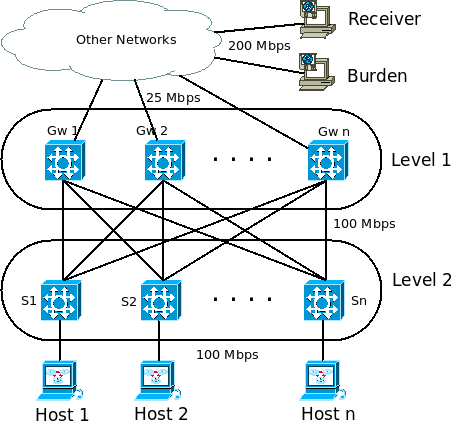
\includegraphics[width=0.6\textwidth]
		{pics/diagram/bipartite.png}
		\caption{Topologi \textit{Bipartite} untuk Pengukuran Fail-Over Delay}
	\label{fig:bipartite}
\end{figure}
\end{lstlisting}

\begin{figure}
	\centering
	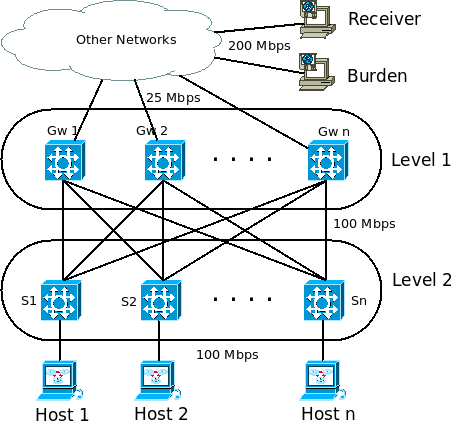
\includegraphics[width=0.6\textwidth]
		{pics/diagram/bipartite.png}
		\caption{Topologi \textit{Bipartite} untuk Pengukuran Fail-Over Delay}
	\label{fig:bipartite}
\end{figure}

\subsection{Membuat Tabel}
Untuk memasukkan tabel ke dalam dokumen, digunakan \textit{syntax} \textbackslash begin\{table\} ... \textbackslash end\{table\}

\begin{lstlisting}
\begin{table}
	\centering
	\caption{Jumlah \textit{Switch} dan \textit{Host} serta Jenis \textit{Traffic} untuk Setiap Pengukuran}
	\label{tab:tab1}
	\begin{tabular}{| l | r | r | r | c |}
		\hline
		Pengukuran & L1 & L2 & \textit{Host} & \textit{Traffic}\\ 
		\hline
		\textit{Fail-Over Delay} & 2 - 4  & 1 - 8 & 1 - 8 & ICMP Ping Tunggal\\
		\textit{Load Balance: Load Distribution} & 1 - 4 & 1 & 1 & 200 UDP \textit{Flows}\\
		\textit{Load Balance: Performance} & 1 - 4  & 1 - 8 & 1 - 8 & Data, Video, VoIP \textit{Flows}\\
		\textit{Overhead Size} & 2 & 1 & 1 & 25 - 150 UDP \textit{Flows}\\
		\textit{Memory Consumption: Switch} & 1 - 4  & 1 - 8 & 0 & -\\
		\textit{Memory Consumption: Host}  & 1 & 1 & 0 - 200 & - \\
		\hline
	\end{tabular}
\end{table}
\end{lstlisting}

\begin{table}
	\centering
	\caption{Jumlah \textit{Switch} dan \textit{Host} serta Jenis \textit{Traffic} untuk Setiap Pengukuran}
	\label{tab:tab1}
	\begin{tabular}{| l | r | r | r | c |}
		\hline
		Pengukuran & L1 & L2 & \textit{Host} & \textit{Traffic}\\ 
		\hline
		\textit{Fail-Over Delay} & 2 - 4  & 1 - 8 & 1 - 8 & ICMP Ping Tunggal\\
		\textit{Load Balance: Load Distribution} & 1 - 4 & 1 & 1 & 200 UDP \textit{Flows}\\
		\textit{Load Balance: Performance} & 1 - 4  & 1 - 8 & 1 - 8 & Data, Video, VoIP \textit{Flows}\\
		\textit{Overhead Size} & 2 & 1 & 1 & 25 - 150 UDP \textit{Flows}\\
		\textit{Memory Consumption: Switch} & 1 - 4  & 1 - 8 & 0 & -\\
		\textit{Memory Consumption: Host}  & 1 & 1 & 0 - 200 & - \\
		\hline
	\end{tabular}
\end{table}

\subsection{Notasi Matematika}
Untuk menuliskan notasi matematika, pada \latex digunakan \textit{syntax} \$ ... \$ untuk penggunaan di dalam paragraf dan \textbackslash begin\{equation\} ... \textbackslash end\{equation\} untuk penggunaan terpisah di luar paragraf. Sebagai contoh sebagai berikut.
\begin{itemize}
\item contoh 1:
\begin{lstlisting}
\begin{equation}
	metric_{i,j} = \frac{10^2}{(capacity_{E_{i,j}} - 	load_{E_{i,j}})}
	\label{eq:metric1}
\end{equation}
\end{lstlisting}
\begin{equation}
	metric_{i,j} = \frac{10^2}{(capacity_{E_{i,j}} - 	load_{E_{i,j}})}
	\label{eq:metric1}
\end{equation}
\item contoh 2:
\begin{lstlisting}
\begin{equation}
	f(x)=(x+a)(x+b)
	\label{eq:fx1}
\end{equation}
\end{lstlisting}
\begin{equation}
	f(x)=(x+a)(x+b)
	\label{eq:fx1}
\end{equation}
\item contoh 3
\begin{lstlisting}
\begin{subequations}
Maxwell's equations:
	\begin{align}
		B'&=-\nabla \times E,\\
		E'&=\nabla \times B - 4\pi j,
	\end{align}
	\label{eq:maxwell}
\end{subequations}
\end{lstlisting}
\begin{subequations}
Maxwell's equations:
	\begin{align}
		B'&=-\nabla \times E,\\
		E'&=\nabla \times B - 4\pi j,
	\end{align}
	\label{eq:maxwell}
\end{subequations}
\item contoh 4
\begin{lstlisting}[language=tex]
matriks $Adj$ digunakan untuk menggambarkan topologi jaringan  $G = (V,E)$, di mana $V = \{v_{1}, v_{2}, ..., v_{n}\}$ merupakan \textit{switch} dan $E = \{e_{1,1}, e_{1,2}, ..., e_{n,n}\}$ merupakan \textit{link} antar-\textit{switch}. Setiap $E_{i,j}$ menyimpan informasi \textit{metric} sesuai persamaan \ref{eq:metric1} . Hasil dari algoritma ini adalah jalur $T_{k,l}$ yang disimpan di dalam \textit{bucket Path} atau $T$. Setiap $T_{k,l}$ mempunyai nilai \textit{metric} sesuai persamaan \ref{eq:metric2}.
\end{lstlisting}
matriks $Adj$ digunakan untuk menggambarkan topologi jaringan  $G = (V,E)$, di mana $V = \{v_{1}, v_{2}, ..., v_{n}\}$ merupakan \textit{switch} dan $E = \{e_{1,1}, e_{1,2}, ..., e_{n,n}\}$ merupakan \textit{link} antar-\textit{switch}. Setiap $E_{i,j}$ menyimpan informasi \textit{metric} sesuai persamaan \ref{eq:metric1}. Hasil dari algoritma ini adalah jalur $T_{k,l}$ yang disimpan di dalam \textit{bucket Path} atau $T$. Setiap $T_{k,l}$ mempunyai nilai \textit{metric} sesuai persamaan 3.2.
\end{itemize} 

\subsection{Notasi Algoritma \textit{Pseudo-Code}}
Untuk menuliskan \textit{pseudo-code} digunakan \textit{syntax} \textbackslash begin\{algorithm\} ... \textbackslash end\{algorithm\}. Berikut contoh notasi \textit{pseudo code}.
\begin{lstlisting}
\begin{algorithm}
\caption{--- Find all possible path from graph G --- Adapted from DFS algorithm}\label{alg1}
\begin{algorithmic}[1]
\Require network topology $G = (V,E)$ represented in dictionary $Adj$, where $V, E$ represents DPID and link between DPID
\Ensure a routing table for source-destination DPID pairs represented in dictionary $T$
\State $T \leftarrow \{\}$
\Procedure{Per\textunderscore Source\textunderscore DFS}{$source, origin =$ None, $path \leftarrow []$}
  \If{$origin \equiv$ None}
    \State $origin \leftarrow source$
  \EndIf
  \For{$i \in M[source]$}
    \If{$i \in path \lor i \equiv origin$}
      \State continue
    \Else
      \If{$i \notin T[origin]$}
        \State $T[origin][i] \leftarrow [path + [i])]$
        \Else
          \State append $[path + [i])]$ to $T[origin][i]$
      \EndIf
      \State PER\textunderscore SOURCE\textunderscore DFS($i, origin, path + [i]$)
    \EndIf
  \EndFor
\EndProcedure
\For{$i \in Adj$}
  \State $path[i] \leftarrow \{\}$
  \State PER\textunderscore SOURCE\textunderscore DFS($i$)
\EndFor
\end{algorithmic}
\end{algorithm}
\end{lstlisting}

\begin{algorithm}
\caption{--- Find all possible path from graph G --- Adapted from DFS algorithm}\label{alg1}
\begin{algorithmic}[1]
\Require network topology $G = (V,E)$ represented in dictionary $Adj$, where $V, E$ represents DPID and link between DPID
\Ensure a routing table for source-destination DPID pairs represented in dictionary $T$
\State $T \leftarrow \{\}$
\Procedure{Per\textunderscore Source\textunderscore DFS}{$source, origin =$ None, $path \leftarrow []$}
  \If{$origin \equiv$ None}
    \State $origin \leftarrow source$
  \EndIf
  \For{$i \in M[source]$}
    \If{$i \in path \lor i \equiv origin$}
      \State continue
    \Else
      \If{$i \notin T[origin]$}
        \State $T[origin][i] \leftarrow [path + [i])]$
        \Else
          \State append $[path + [i])]$ to $T[origin][i]$
      \EndIf
      \State PER\textunderscore SOURCE\textunderscore DFS($i, origin, path + [i]$)
    \EndIf
  \EndFor
\EndProcedure
\For{$i \in Adj$}
  \State $path[i] \leftarrow \{\}$
  \State PER\textunderscore SOURCE\textunderscore DFS($i$)
\EndFor
\end{algorithmic}
\end{algorithm}

\subsection{Penulisan Daftar Referensi}
Terdapat banyak sekali gaya penulisan daftar referensi. Pada \textit{template} ini penulisan daftar referensi merujuk ke IEEE. Gaya penulisan daftar referensi IEEE \cite{ieee_style} memiliki beberapa format yang berbeda untuk jenis referensi yang berbeda. Jenis-jenis publikasi yang diterangkan cara penulisan daftar referensinya oleh IEEE antara lain: \textit{paper} jurnal, \textit{paper} seminar/\textit{conference}, dokumen paten, dokumen standar, dokumen laporan/\textit{report}, tesis dan disertasi, buku, serta beberapa dokumen, artikel, perangkat lunak, maupun sumber kode yang tersedia \textit{online}. Pada \textit{pustaka.tex}, sudah dibuat beberapa daftar referensi sebagai contoh dalam pembuatan daftar referensi lain yang diinginkan oleh penulis.


% Bab 4 : Pengujian
%-----------------------------------------------------------------------------%
\chapter{\babEmpat}
%-----------------------------------------------------------------------------%

%-----------------------------------------------------------------------------%
\section{Petunjuk Penggunaan}
%-----------------------------------------------------------------------------%

\textit{Template} tugas akhir ini dibuat menggunakan \latex. Oleh karena itu, dibutuhkan \latex~\textit{builder} untuk mengolah kode yang sudah dibuat. Hasil dari proses \textit{build} adalah \textit{file} PDF (\textit{portable document format}), bukan \textit{.odt} maupun \textit{.doc}. Sehingga dibutuhkan aplikasi PDF \textit{reader} untuk membuka pdf hasil pengolahan kode yang dibuat. Beberapa kode-kode yang dapat digunakan di dalam \textit{template} ini sudah ditunjukkan pada bab3 sesuai dengan contohnya masing-masing.

Lankah paling awal untuk menggunakan \textit{template} ini adalah memodifikasi \textit{konfigurasi.tex}. Modifikasi ini dilakukan dengan merubah nilai-nilai variabel yang terdapat di dalam berkas \textit{konfigurasi.tex}, sehingga nilainya sesuai dengan yang penulis inginkan. Nilai variabel-variabel yang diganti tersebut akan merubah isi berkas pdf, setelah kode-kode tersebut diproses. Untuk memproses \textit{template} ini, penulis hanya perlu men-\textit{build} \textit{main.tex}. Berkas-berkas \textit{.tex} lain akan secara otomatis ter-\textit{build}~juga ketika \textit{main.tex} di-\textit{build}.

Selanjutnya penulis dapat memulai proses penulisan atau pengisian buku. Berkas-berkas yang perlu dirubah antara lain \textit{abstrak.tex, abstract.tex}~berisi abstrak berbahasa Inggris dan Indonesia, \textit{pengantar.tex} berisi kata pengantar, \textit{bab1.tex} hingga \textit{bab5.tex} diisi sesuai yang penulis inginkan, serta \textit{pustaka.tex} untuk memasukkan daftar pustaka.

\begin{figure}
	\centering
	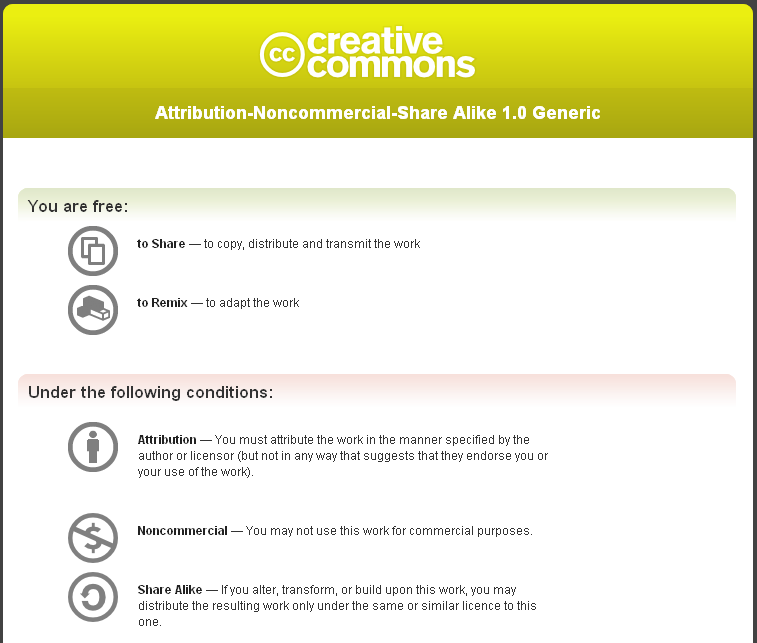
\includegraphics[width=0.3\textwidth]
		{pics/creative_common.png}
		\caption{CC-A-NC-SA 1.0 Generic}
	\label{fig:CC10}
\end{figure}

\textit{Template} tugas ini dipasangkan lisensi \textit{Creative Common---Attribution---Non Commercial---Share Alike 1.0 Generic}.

% Bab 5 : Kesimpulan dan Saran
%---------------------------------------------------------------
\chapter{\babLima}
%---------------------------------------------------------------

%---------------------------------------------------------------
\section{Kesimpulan}
%---------------------------------------------------------------

%---------------------------------------------------------------
\section{Saran}
%---------------------------------------------------------------


%
% Daftar Pustaka
%
% Daftar Pustaka 
% 

% 
% Tambahkan pustaka yang digunakan setelah perintah berikut. 
% 
\begin{thebibliography}{99}

\bibitem{per_journal}
{J. K. Author, “Name of paper,” \textit{Abbrev. Title of Periodical}, vol. x, no. x, pp. xxx-xxx, Abbrev. Month, year.}

\bibitem{per_journal_1}
{S. Azodolmolky et al., Experimental demonstration of an impairment aware network planning and operation tool for transparent/translucent optical networks ,” \textit{J. Lightw. Technol.}, vol. 29, no. 4, pp. 439–448, Sep. 2011.}

\bibitem{per_journal_2}
{J. Zhang and N. Tansu, “Optical gain and laser characteristics of InGaN quantum wells on ternary InGaN substrates,” \textit{IEEE Photon. J.}, vol. 5, no. 2, Apr. 2013, Art. ID 2600111.}

\bibitem{per_journal_3}
{W. Rafferty, “Ground antennas in NASA’s deep space telecommunications,” \textit{Proc. IEEE}, vol. 82, no. 5, pp. 636-640, May 1994.}

\bibitem{book}
{J. K. Author, “Title of chapter in the book,” in \textit{Title of His Published Book}, xth ed. City of Publisher, (only U.S. State), Country: Abbrev. of Publisher, year, ch. x, sec. x, pp. xxx–xxx.}

\bibitem{book_1}
{R. Ramaswami, K. N. Sivarajan, and G. H. Sasaki, \textit{Optical Network: A Practical Prespective}, 3rd ed. Burlington, MA, USA: Elsevier, 2010.}

\bibitem{report}
{J. K. Author, “Title of report,” Abbrev. Name of Co., City of Co., Abbrev. State, Country, Rep. xxx, year.}

\bibitem{report_1}
{M. Chui et al, "The Social Economy: Unlocking Value and Productivity Through Social Technologies", McKinsey Global Institute, 2012.}

\bibitem{conference}
{J. K. Author, “Title of paper,” in \textit{Abbreviated Name of Conf}., (location of conference is optional), year, pp. xxx-xxx.}

\bibitem{conference_1}
{B. Lantz, B. Heller dan N. McKeown, "A Network in a Laptop: Rapid Prototyping for Software-defined Networks"., dalam \textit{Proceedings of the 9th ACM SIGCOMM Workshop on Hot Topics in Networks}, New York, 2010.}

\bibitem{conference_2}
{A. Sefano, D. Emma, A. Pescape dan G. Ventre, "A Practical Demonstration of Network Traffic Generation"., dalam \textit{Proceedings of the 8th IASTED International Conference}, Hawaii, 2004, pp. 138-143.}

\bibitem{paten}
{J. K. Author, “Title of patent,” U.S. Patent x xxx xxx, Abbrev. Month, day, year.}

\bibitem{paten_1}
{S. P. Voinigescu et al., "Direct m-ary quadrature amplitude modulation (QAM) operating in saturated power mode,” U.S. Patent Appl. 20110013726A1, Jan. 20, 2011.}

\bibitem{theses}
{J. K. Author, “Title of thesis,” M.S. thesis, Abbrev. Dept., Abbrev. Univ., City of Univ., Abbrev. State, year.}

\bibitem{dissertation}
{J. K. Author, “Title of dissertation,” Ph.D. dissertation, Abbrev. Dept., Abbrev. Univ., City of Univ., Abbrev. State, year.}

\bibitem{theses_1}
{N. Kawasaki, “Parametric study of thermal and chemical nonequilibrium nozzle flow,” M.S. thesis, Dept. Electron.
Eng., Osaka Univ., Osaka, Japan, 1993.}

\bibitem{theses_2}
{B. Joaquim, "Redundancy and Load Balancing at IP layer in Access and Aggregation Networks", Master Thesis, Aalto University. 2011}

\bibitem{thesis_2}
{S. Ejaz, "Analysis of the trade-off between performance and energy consumption of existing load balancing algorithms", Grober Beleg, Technische Universitat Dresden, 2011.}

\bibitem{standard}
{\textit{Title of Standard}, Standard number, date.}

\bibitem{standard_1}
{\textit{Software-Defined Networking: The New Norm for Networks}, Open Network Foundation, 2012.}

\bibitem{standard_2}
{\textit{Virtual Router Redundancy Protocol (VRRP) Version 3 for IPv4 and IPv6}. IETF RFC 5798. 2010.}

\bibitem{manual}
T. Antcom, CA, USA. Antenna Products. (2011) [Online]. Tersedia di http://www.antcom.com/documents/catalogs /L1L2GPSAntennas.pdf, Diakses pada 12 Februari 2014.

\bibitem{software_source_code}
Drox. (2015) [Online]. Tersedia di \url{http://github.com/haidlir/drox}, Diakses pada 26 Juli 2015.

\bibitem{Artikel}
{T. Oetiker. The Not So Short Introduction to \latex2ε. (2014) [Online]. Tersedia di \url{https://tobi.oetiker.ch/lshort/lshort.pdf}. 
Diakses pada 8 Mei 2015.}

\bibitem{ta_panduan}
{Format Penulisan Buku Tugas Akhir S1. (2011) [Online]. Tersedia di \url{http://www.ee.itb.ac.id/format_penulisan_buku_tugas_akhir_s1}. Diakses pada 26 Juli 2015.}

\bibitem{ieee_style}
{IEEE Editorial Style Manual. (2014) [Online]. Tersedia di \url{https://www.ieee.org/documents/style_manual.pdf}. Diakses pada 25 Juli 2015.}

\end{thebibliography}
%\bibliographystyle{plain}
%\bibliography{ref}

% Lampiran 
\begin{appendix}
	\pagenumbering{gobble}
	%
% @author  Andreas Febrian
% @version 1.00 
% 
% Hanya sebuah pembatas bertuliskan LAMPIRAN ditengah halaman. 
% 

\begin{titlepage}
	\centering 
	\vspace*{6cm}
	\noindent \Huge{LAMPIRAN}
	\addChapter{LAMPIRAN}
\end{titlepage}
%	\setcounter{page}{2}
\end{appendix}

\end{document}